% Asset ID: AS1AlgebraicMethodsTikZ-002
% Unit code: AS1
% Topic code: AS1-AF
% Topic ID: AS1AlgebraicMethodsFactorTheorem
% Related LO IDs: AS1-AF-LO011
% Source: CCEA Mathematics Specification Map; Chapter 7a Algebraic Methods transcript
% Related lesson section: Core Theory F-I: Remainder Theorem, Factor Theorem and Unknown Coefficients
% Purpose: Provide a compact printable TikZ decision card linking divisor form, substitution value, remainder theorem and factor theorem.
% Note: This is an AI-proposed teaching enhancement based on the CCEA boundary and evidence-backed methods.

\documentclass[tikz,border=8pt]{standalone}
\usepackage{amsmath}
\usepackage{amssymb}
\usetikzlibrary{arrows.meta, positioning}
\begin{document}
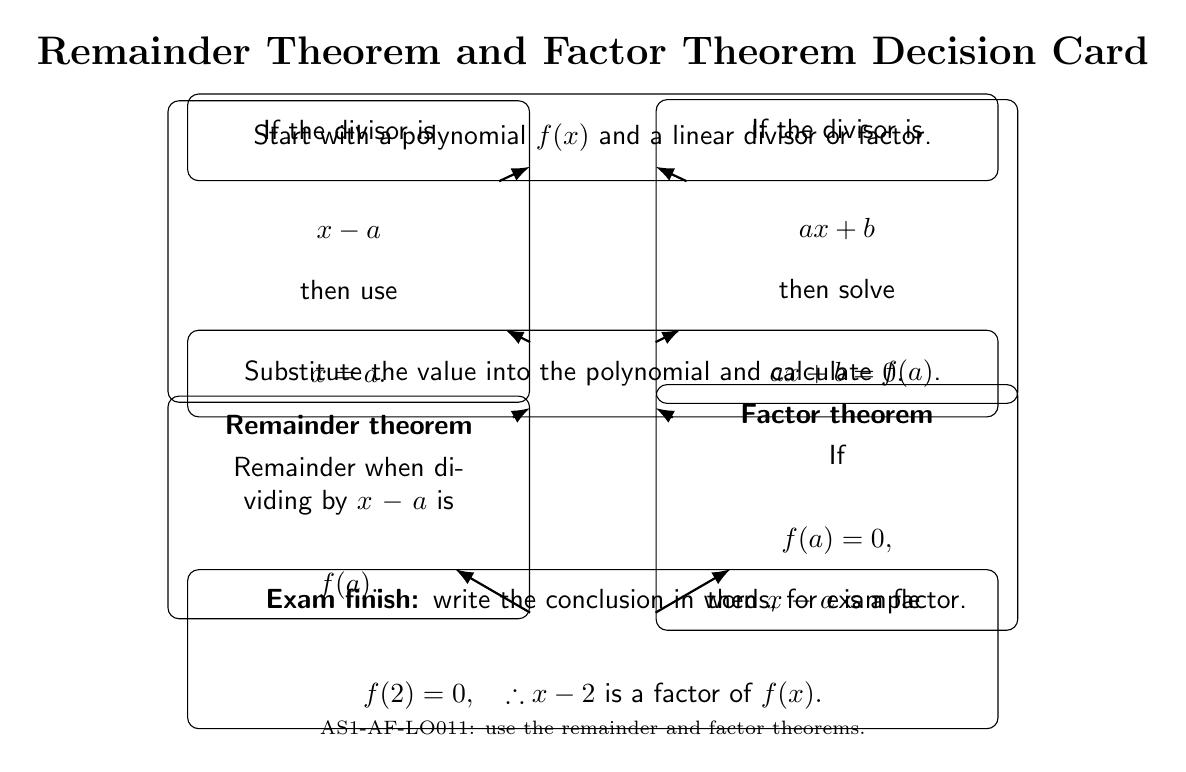
\begin{tikzpicture}[
    every node/.style={font=\sffamily},
    box/.style={draw,rounded corners=4pt,align=center,text width=4.1cm,minimum height=1.25cm,inner sep=7pt},
    widebox/.style={draw,rounded corners=4pt,align=center,text width=9.8cm,minimum height=1.1cm,inner sep=7pt},
    arrow/.style={-Latex, thick}
]
\node[font=\bfseries\Large] at (0,4.25) {Remainder Theorem and Factor Theorem Decision Card};
\node[widebox] (start) at (0,3.15) {Start with a polynomial \(f(x)\) and a linear divisor or factor.};
\node[box] (xa) at (-3.1,1.7) {If the divisor is\\[2pt] \[x-a\] then use\\[-4pt] \[x=a.\]};
\node[box] (axb) at (3.1,1.7) {If the divisor is\\[2pt] \[ax+b\] then solve\\[-4pt] \[ax+b=0.\]};
\node[widebox] (sub) at (0,0.15) {Substitute the value into the polynomial and calculate \(f(a)\).};
\node[box] (rem) at (-3.1,-1.55) {\textbf{Remainder theorem}\\[3pt] Remainder when dividing by \(x-a\) is\\[-4pt] \[f(a).\]};
\node[box] (fac) at (3.1,-1.55) {\textbf{Factor theorem}\\[3pt] If\\[-4pt] \[f(a)=0,\] then \(x-a\) is a factor.};
\node[widebox] (exam) at (0,-3.35) {\textbf{Exam finish:} write the conclusion in words, for example\\ \[f(2)=0,\quad \therefore x-2\text{ is a factor of }f(x).\]};
\draw[arrow] (start) -- (xa);
\draw[arrow] (start) -- (axb);
\draw[arrow] (xa) -- (sub);
\draw[arrow] (axb) -- (sub);
\draw[arrow] (sub) -- (rem);
\draw[arrow] (sub) -- (fac);
\draw[arrow] (rem) -- (exam);
\draw[arrow] (fac) -- (exam);
\node[font=\scriptsize] at (0,-4.35) {AS1-AF-LO011: use the remainder and factor theorems.};
\end{tikzpicture}
\end{document}
